% Fitting gamma-ray spectra: an explainer for the Gamma Line Explorer fitter.
% Build:  node figdata.js > figdata.json && python3 figures.py && latexmk -pdf gammafit.tex
% (or simply: make).  The figures are drawn from the site's own fit engine, assets/gammafit-core.js.
\documentclass[11pt]{article}
\usepackage[letterpaper,margin=1in]{geometry}
\usepackage[T1]{fontenc}
\usepackage{lmodern}
\usepackage{microtype}
\usepackage{amsmath,amssymb,mathtools,bm}
\usepackage{siunitx}
\usepackage{graphicx}
\usepackage{booktabs,array,tabularx}
\usepackage{xcolor}
\usepackage{enumitem}
\usepackage{caption}
\usepackage[section]{placeins}
\usepackage[most]{tcolorbox}
\usepackage{listings}
\usepackage[ruled,vlined,linesnumbered]{algorithm2e}
\usepackage{tikz}
\usetikzlibrary{arrows.meta,positioning,shapes.geometric,fit,calc}
\usepackage[colorlinks=true,linkcolor=blue!50!black,citecolor=blue!50!black,urlcolor=blue!50!black]{hyperref}
\usepackage[capitalise,noabbrev]{cleveref}

\sisetup{group-separator={,},group-minimum-digits=4}
\definecolor{labblue}{HTML}{0088EE}
\definecolor{codebg}{HTML}{F6F8FA}
\definecolor{exbg}{HTML}{FFF7EC}
\definecolor{boxbg}{HTML}{EEF4FB}

\newtcolorbox{keyidea}[1][]{colback=boxbg,colframe=labblue,boxrule=0.6pt,arc=2pt,left=6pt,right=6pt,top=4pt,bottom=4pt,fonttitle=\bfseries,title={#1}}
\newtcolorbox{pitfall}[1][]{colback=red!3,colframe=red!55!black,boxrule=0.6pt,arc=2pt,left=6pt,right=6pt,top=4pt,bottom=4pt,fonttitle=\bfseries,title={#1}}
\newcounter{exercise}[section]
\renewcommand{\theexercise}{\thesection.\arabic{exercise}}
\newtcolorbox{exercise}[1][]{colback=exbg,colframe=orange!70!black,boxrule=0.6pt,arc=2pt,left=6pt,right=6pt,top=4pt,bottom=4pt,fonttitle=\bfseries,
  title={Exercise~\refstepcounter{exercise}\theexercise\ifx\relax#1\relax\else\ (#1)\fi}}

\lstdefinelanguage{JavaScript}{keywords={var,function,return,if,else,for,while,new,this,true,false,null},
  morecomment=[l]{//},morecomment=[s]{/*}{*/},morestring=[b]',morestring=[b]"}
\lstset{basicstyle=\ttfamily\footnotesize,backgroundcolor=\color{codebg},frame=single,rulecolor=\color{black!15},
  keywordstyle=\color{blue!60!black}\bfseries,commentstyle=\color{black!55}\itshape,stringstyle=\color{orange!60!black},
  breaklines=true,columns=fullflexible,keepspaces=true,showstringspaces=false,xleftmargin=2pt,xrightmargin=2pt,aboveskip=6pt,belowskip=6pt}

\newcommand{\dd}{\mathrm{d}}
\newcommand{\E}{\mathbb{E}}
\newcommand{\keV}{\,\mathrm{keV}}
\newcommand{\T}{^{\mathsf{T}}}
\newcommand{\vth}{\bm{\theta}}
\newcommand{\vx}{\bm{x}}
\newcommand{\vmu}{\bm{\mu}}
\newcommand{\vn}{\bm{n}}
\newcommand{\code}[1]{\texttt{#1}}
\newcommand{\nuc}[2]{${}^{#1}$#2}

\title{\textbf{Fitting Gamma-Ray Spectra}\\[4pt]
\large Response functions, Poisson likelihoods and the algorithms behind the\\ Gamma Line Explorer spectrum fitter}
\author{UCR Dark Matter Group\\\small\url{https://dark-matter.ucr.edu} \quad Source: \url{https://github.com/UCRDarkMatter/dark-matter-lab-site}}
\date{November 2026}

\begin{document}
\maketitle

\begin{abstract}
\noindent
A gamma-ray spectrum is a histogram of energy deposits. The gamma lines that caused it are hidden behind a detector that blurs, scatters and loses part of every photon. This document explains, from first principles, how the Gamma Line Explorer's fitter recovers which sources are present and how strong they are. It covers what a detector response function is and how it is built (from physics, from a parameterized model, or from a simulation). It covers why gamma spectra must be fitted with a Poisson likelihood, and how that likelihood is maximized: an expectation-maximization algorithm for the many non-negative amplitudes, and Levenberg--Marquardt with variable projection for the few nonlinear response parameters. It also covers how sources are selected and how uncertainties are assigned. Each step is tied to the code that implements it, and each section ends with exercises. Together the exercises take a graduate student from deriving the Compton edge to writing and validating a forward-folding fitter of their own. A short reference implementation (about 140 lines) in Python is included.
\end{abstract}

\tableofcontents
\newpage

%=====================================================================
\section{How to use this document}
%=====================================================================
The fitter lives in a single file, \code{assets/gammafit-core.js} (about 500 lines), which runs in a background thread of the browser. The user interface is in \code{assets/gammas.js}. The shorter user guide is \code{GammasGuide.html}. Every figure in this document was produced by running that same engine (\code{docs/gammafit/figdata.js}), so what you see is what the web page does. The \LaTeX{} source, figure scripts and the teaching implementation \code{minifit.py} are in \code{docs/gammafit/} of the repository.

The material is ordered the way you would build a fitter yourself:
\begin{enumerate}[nosep]
\item the measurement and its statistics (\cref{sec:measurement});
\item the response function: physics, models and simulations (\cref{sec:response});
\item the full model of a spectrum and the likelihood (\cref{sec:likelihood});
\item solving for the amplitudes (\cref{sec:mlem}) and the response parameters (\cref{sec:theta});
\item choosing sources (\cref{sec:selection}) and quoting uncertainties (\cref{sec:uncertainty});
\item implementation, validation and limits (\cref{sec:implementation,sec:validation,sec:limits}).
\end{enumerate}
Exercises are marked by difficulty: \emph{(A)} analytic, \emph{(P)} programming, \emph{(R)} research-style and open-ended. A suggested capstone project is in \cref{sec:capstone}.

\begin{table}[h]
\centering\small
\caption{Notation used throughout.}\label{tab:notation}
\begin{tabularx}{\linewidth}{@{}lX@{}}
\toprule
$i = 1\dots N$ & channel (bin) index; $E_i$ its centre energy, $\Delta E_i$ its width\\
$n_i$ & observed counts in channel $i$\\
$\mu_i$ & expected counts in channel $i$ (the model)\\
$E_\gamma$, $E'$ & true gamma energy; energy deposited in the detector\\
$R(E'\mid E_\gamma)$ & response: probability density of depositing $E'$ per emitted gamma of energy $E_\gamma$\\
$k$ & candidate source (a nuclide or a group in equilibrium); $\ell$ its lines, with energies $E_{k\ell}$ and intensities $I_{k\ell}$ per decay\\
$A_k$ & amplitude of source $k$ (proportional to its number of decays)\\
$\beta_j$, $B_j$ & background amplitudes and B-spline basis functions\\
$T_{ik}(\vth)$ & template: expected counts in channel $i$ per unit amplitude of source $k$\\
$\vx = (\bm\beta,\bm A)$ & all linear amplitudes, constrained to $\vx \ge 0$\\
$\vth$ & nonlinear response parameters (calibration, resolution, efficiency, shape)\\
$\theta^0_a \pm \sigma_a$ & Gaussian prior on parameter $\theta_a$\\
$D$ & Poisson deviance (likelihood-ratio $\chi^2$)\\
\bottomrule
\end{tabularx}
\end{table}

%=====================================================================
\section{The measurement}\label{sec:measurement}
%=====================================================================
A spectroscopy system converts each detected photon interaction into a pulse whose height is (ideally) proportional to the energy deposited, then sorts pulse heights into $N$ channels. Over a live time $t$ the number of events in channel $i$ is a sum of a huge number of rare, independent events, so
\begin{equation}
n_i \sim \mathrm{Poisson}(\mu_i), \qquad P(n_i\mid\mu_i) = \frac{\mu_i^{n_i}e^{-\mu_i}}{n_i!}, \label{eq:poisson}
\end{equation}
independently for every channel. Two features dominate everything that follows. First, $\mathrm{Var}(n_i) = \mu_i$: the noise depends on the \emph{model}, not on the data. Second, low-count channels are common (a long background run in a shielded HPGe detector has many empty channels above \SI{2}{MeV}), and there the Poisson distribution is strongly skewed.

Channels map to energy through a \emph{calibration}, here a polynomial
\begin{equation}
E(\mathrm{ch}) = c_0 + c_1\,\mathrm{ch} + c_2\,\mathrm{ch}^2,\qquad \Delta E_i = E(i+\tfrac12) - E(i-\tfrac12). \label{eq:calib}
\end{equation}
For a scintillator read out with photomultipliers, $c_1$ is set by the light yield and the electronics gain. With an x-axis in photoelectrons, $1/c_1$ \emph{is} the light yield in photoelectrons per keV. The fitter treats $c_0,c_1,c_2$ as parameters to be fitted with priors (\cref{sec:theta}), because a spectrum contains its own calibration information: the positions of known lines.

\begin{keyidea}[Forward folding versus unfolding]
There are two ways to connect a spectrum to sources. \emph{Unfolding} inverts the detector: it estimates the incident photon spectrum $S(E_\gamma)$ from the measured $n_i$. That is an ill-posed inverse problem that needs regularization. \emph{Forward folding} goes the other way: propose sources and a detector, predict $\mu_i$, compare with $n_i$. The fitter forward-folds. It never inverts the response, it uses the exact counting statistics, and the candidate list (from the nuclear data and the experimental setup) acts as a very strong, physically meaningful regularizer: only real gamma lines are allowed.
\end{keyidea}

\begin{exercise}[A]
Show that for $\mu \gg 1$ the Poisson distribution approaches a Gaussian with mean and variance $\mu$. For $\mu = 3$, compute $P(n=0)$ and compare with the Gaussian approximation. In which channels of a typical spectrum does the difference matter?
\end{exercise}

\begin{exercise}[A]
A channel has $n=0$ counts. What does the Neyman $\chi^2 = \sum (n_i-\mu_i)^2/n_i$ do with it? Explain why many codes then substitute $n_i \to \max(n_i,1)$, and why this biases the fitted peak areas low. (We return to this in \cref{sec:likelihood}.)
\end{exercise}

%=====================================================================
\section{The detector response function}\label{sec:response}
%=====================================================================
\subsection{Definition}
The \emph{response function} $R(E'\mid E_\gamma)$ is the probability density that a photon of energy $E_\gamma$, emitted from the source position, deposits energy $E'$ in the detector, \emph{per emitted photon}. If the source emits a photon spectrum $S(E_\gamma)$ (photons per keV during the measurement), the expected spectrum is the folding integral
\begin{equation}
\mu(E') = \int R(E'\mid E_\gamma)\,S(E_\gamma)\,\dd E_\gamma, \qquad
\mu_i = \int_{E_i-\Delta E_i/2}^{E_i+\Delta E_i/2}\mu(E')\,\dd E'. \label{eq:fold}
\end{equation}
For radioactive sources $S$ is a sum of lines, $S(E_\gamma) = \sum_k \mathcal N_k \sum_\ell I_{k\ell}\,\delta(E_\gamma - E_{k\ell})$, with $\mathcal N_k$ decays and $I_{k\ell}$ photons per decay. The integral collapses to a sum:
\begin{equation}
\mu_i = \sum_k \mathcal N_k \underbrace{\sum_\ell I_{k\ell}\,\bar R_i(E_{k\ell})}_{T_{ik}},\qquad \bar R_i(E_\gamma) = \int_{\text{bin } i} R(E'\mid E_\gamma)\,\dd E'. \label{eq:template}
\end{equation}
$T_{ik}$ is the \emph{template} of source $k$: what one decay contributes to each channel. The task of modelling a detector is the task of computing $\bar R_i(E_\gamma)$ for any line energy. The integral of $R$ over all $E'>0$ is the \emph{total efficiency} $\varepsilon_\text{tot}(E_\gamma)$. The integral over the full-energy peak alone is the \emph{photopeak efficiency} $\varepsilon_\text{pk}$. Their ratio is the \emph{peak-to-total ratio} $P/T$.

\subsection{The physics that shapes $R$}
Three interactions matter between \SI{50}{keV} and \SI{3}{MeV}.

\paragraph{Photoelectric absorption.} The photon is absorbed and its whole energy (less binding energy, which is then recovered as X-rays and Auger electrons in all but small detectors) is deposited, giving the \emph{full-energy peak}. It dominates at low energy and in high-$Z$ materials (cross section $\propto Z^{4\text{--}5}/E_\gamma^{3}$).

\paragraph{Compton scattering.} The photon scatters off an electron and leaves with reduced energy. With $\epsilon = E_\gamma/m_ec^2$ and scattering angle $\vartheta$,
\begin{equation}
E_\gamma' = \frac{E_\gamma}{1+\epsilon(1-\cos\vartheta)},\qquad T = E_\gamma - E_\gamma'. \label{eq:compton}
\end{equation}
The electron recoil energy $T$ ranges from 0 to the \emph{Compton edge} $T_\text{max} = E_\gamma\,2\epsilon/(1+2\epsilon)$ (at $\vartheta=\pi$). The photon that scatters back by $\approx 180^\circ$ in material \emph{around} the detector and is then absorbed produces the \emph{backscatter peak} at $E_\gamma/(1+2\epsilon)$, which is about \SIrange{200}{250}{keV} for any line above \SI{1}{MeV}. The distribution of $T$ for a single scatter follows from the Klein--Nishina cross section~\cite{KleinNishina}:
\begin{equation}
\frac{\dd\sigma}{\dd T} = \frac{\pi r_e^2}{m_ec^2\epsilon^2}\left[2 + \frac{s^2}{\epsilon^2(1-s)^2} + \frac{s}{1-s}\left(s-\frac{2}{\epsilon}\right)\right],\qquad s = \frac{T}{E_\gamma}, \label{eq:kn}
\end{equation}
which is what \code{kn(E, T)} evaluates (without the constant prefactor). \Cref{fig:kn} shows its characteristic shape: roughly flat with a rise into a sharp edge.

\paragraph{Pair production.} Above $2m_ec^2 = \SI{1022}{keV}$ the photon can convert into an $e^+e^-$ pair in the nuclear field. The positron annihilates into two \SI{511}{keV} photons. If one or both escape, the deposit is $E_\gamma - 511$ (\emph{single escape}) or $E_\gamma - 1022$ (\emph{double escape}). This matters mainly for the \SI{2614.5}{keV} line of \nuc{208}{Tl} and for capture gammas.

\begin{figure}[tbp]
\centering
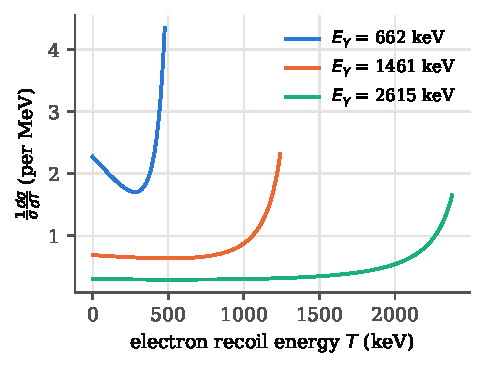
\includegraphics[width=0.48\linewidth]{fig/kn.pdf}\hfill
\begin{minipage}[b]{0.48\linewidth}
\caption{Klein--Nishina distribution of the electron recoil energy for three common lines, each normalized to unit area over $0 < T < T_\text{max}$. The sharp drop is the Compton edge; it is what you see in a small detector where a photon usually scatters once and escapes.}\label{fig:kn}
\end{minipage}
\end{figure}

Real detectors add \emph{multiple Compton scattering}: a photon scattering two or more times before escaping deposits energies between the Compton edge and the photopeak, filling the gap. It also adds escaping secondary electrons and bremsstrahlung, X-ray escape after photoabsorption in iodine or germanium, and \emph{incomplete charge collection}. In a germanium crystal, a small fraction of the charge from photopeak events can be lost to traps, which produces a low-energy tail and a step under each peak.

\subsection{Energy resolution}
Every deposit is measured with a finite resolution. The fitter assumes a Gaussian whose full width at half maximum depends on energy as
\begin{equation}
\mathrm{FWHM}^2(E) = a^2 + b\,E + c\,E^2. \label{eq:fwhm}
\end{equation}
The three terms have physical meanings. $a$ is energy-independent electronic noise. $b$ is the statistics of the information carriers. For a scintillator with light yield $L$ (photoelectrons per keV) and excess noise factor $f$ of the photosensor, $\sigma^2 = fE/L$, so $b = 2.355^2 f/L \approx 5.55\,f/L$. For a semiconductor, $b = 2.355^2 F w$ with Fano factor $F\approx0.1$ and pair-creation energy $w = \SI{2.96}{eV}$ in germanium, which gives $b\approx\SI{1.6e-3}{keV}$. $c$ captures position-dependent light collection or gain drifts, which scale with $E$.

Because channels have finite width, a peak is integrated over each bin rather than sampled at its centre:
\begin{equation}
\bar G_i(E_0,\sigma) = \frac12\left[\operatorname{erfc}\!\left(\frac{E_i-\frac{\Delta E_i}{2}-E_0}{\sqrt2\,\sigma}\right) - \operatorname{erfc}\!\left(\frac{E_i+\frac{\Delta E_i}{2}-E_0}{\sqrt2\,\sigma}\right)\right], \label{eq:gaussbin}
\end{equation}
which sums to exactly 1 over all channels however narrow the peak is. This is \code{addGauss}:
\begin{lstlisting}[language=JavaScript]
function addGauss(col, g, E0, sig, area) {
  var c = g.index(E0), w = 5 * sig / g.dE[Math.round(c)];     // +-5 sigma window
  for (var i = Math.floor(c - w); i <= Math.ceil(c + w); i++) {
    var a = (g.E[i] - 0.5 * g.dE[i] - E0) / (Math.SQRT2 * sig),
        b = (g.E[i] + 0.5 * g.dE[i] - E0) / (Math.SQRT2 * sig);
    col[i] += area * 0.5 * (erfc(a) - erfc(b));
  }
}
\end{lstlisting}
Some lines are intrinsically broader than the resolution. Gammas emitted in flight after $\alpha$ or neutron reactions are Doppler-broadened, and the code adds $0.001E$ or $0.004E$ in quadrature for such flagged lines.

\begin{exercise}[A]
Derive the Compton edge and the backscatter peak energies from \cref{eq:compton}. Evaluate them for \SIlist{662;1461;2614.5}{keV}. Why is the backscatter peak almost independent of $E_\gamma$ at high energy?
\end{exercise}

\begin{exercise}[A]
A NaI(Tl) detector has a resolution of 7\% FWHM at \SI{662}{keV}, dominated by photoelectron statistics. Estimate its light yield in photoelectrons per keV for $f=1.2$. What resolution do you then expect at \SI{1461}{keV}?
\end{exercise}

\begin{exercise}[P]
Compare the bin-integrated Gaussian \cref{eq:gaussbin} with simply evaluating the Gaussian density at the bin centre and multiplying by $\Delta E$, for $\sigma/\Delta E = 0.3, 1, 3$. What fraction of the area is lost or gained in each case? For which detectors does it matter?
\end{exercise}

\subsection{Model 1: peaks with a smooth background (germanium detectors)}
In an HPGe detector the photopeaks are so narrow (FWHM $\approx$ \SIrange{1}{2}{keV}) that each line's Compton continuum is spread thinly over hundreds of keV. Standard practice, followed by the \code{local} mode, is to model only what is local to each peak and to let a smooth background absorb the sum of all continua (\cref{fig:hpge}):
\begin{equation}
\bar R_i(E_\gamma) = \varepsilon(E_\gamma)\Big[\bar G_i(E_\gamma,\sigma) + h\,\tfrac12\operatorname{erfc}\!\big(\tfrac{E_i-E_\gamma}{\sqrt2\sigma}\big)\Delta E_i + \text{tail} + x(E_\gamma)\big(f_\text{se}\bar G_i(E_\gamma-511) + f_\text{de}\bar G_i(E_\gamma-1022)\big)\Big]. \label{eq:local}
\end{equation}
The step height $h$ is a fraction (parameter \code{step}) of the peak height. The tail is an exponential convolved with the Gaussian. The escape fractions grow with energy as $x(E) = \min[1,(E-1022)/1592]$, so that $f_\text{se},f_\text{de}$ are the fractions at \SI{2614}{keV}. The relative efficiency is
\begin{equation}
\ln\varepsilon(E) = e_1 x + e_2 x^2,\qquad x = \ln(E/\SI{1}{MeV}), \label{eq:eff}
\end{equation}
a standard log-log polynomial~\cite{Knoll}, normalized to 1 at \SI{1}{MeV}. Absolute efficiency is not needed: it is absorbed into the amplitudes.

\begin{figure}[tbp]
\centering
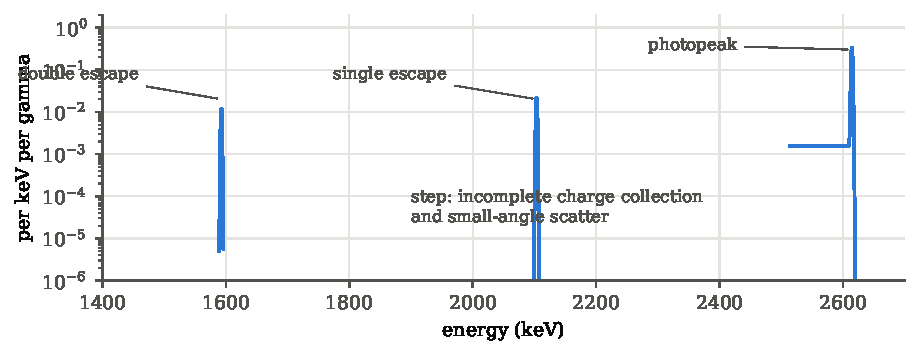
\includegraphics[width=\linewidth]{fig/hpge.pdf}
\caption{Model response of an HPGe detector to the \SI{2614.5}{keV} line in \code{local} mode: bin-integrated Gaussian photopeak, a low-energy step at 0.4\% of the peak height, and single and double escape peaks at 6\% and 3\%. The Compton continuum is deliberately absent: the fitter's smooth background takes it.}\label{fig:hpge}
\end{figure}

\subsection{Model 2: a semi-empirical Compton model (scintillators, liquid nobles)}
In a NaI(Tl), CsI or liquid argon detector the resolution is tens of keV. The Compton continuum of a strong line is then a large, structured part of the spectrum, and a smooth background cannot absorb it without also absorbing peaks. The \code{compton} mode builds the full response of each line from four parts (\cref{fig:anatomy}). Write $p = P/T(E_\gamma)$ and $r = 1-p$:
\begin{align}
\bar R_i(E_\gamma) = \varepsilon(E_\gamma)\Big\{ p\,\bar G_i(E_\gamma) + \mathcal S_\sigma\Big[\, & r(1-f_\text{sh}-f_\text{bs})\,\frac{\dd\sigma/\dd T(E_i)}{\int_0^{T_\text{max}}\dd\sigma/\dd T\,\dd T}\,\Delta E_i \nonumber\\
&+ r f_\text{sh}\,\frac{\mathbb 1[T_\text{max}<E_i<E_\gamma]}{\#\text{bins}} + r f_\text{bs}\,\bar G_i\big(\tfrac{E_\gamma}{1+2\epsilon},\sigma_\text{bs}\big)\Big]\Big\}. \label{eq:compton-model}
\end{align}
Here $\mathcal S_\sigma$ denotes Gaussian smearing with the energy-dependent resolution, and the peak-to-total ratio falls as a power law, $P/T(E) = p_{662}\,(E/\SI{662}{keV})^{-k}$. The shelf models multiple scattering as flat between the edge and the peak. The backscatter peak is given extra width ($8\%$ of its energy) because it comes from a range of angles.

\begin{figure}[tbp]
\centering
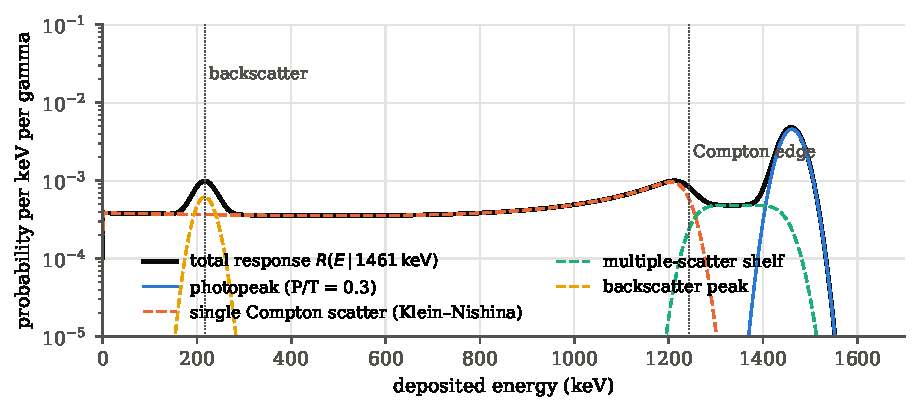
\includegraphics[width=\linewidth]{fig/anatomy.pdf}
\caption{Anatomy of the Compton-model response (\cref{eq:compton-model}) to the \SI{1461}{keV} line of \nuc{40}{K} in a scintillator with $\mathrm{FWHM}\approx\SI{62}{keV}$, computed by the fitter's \code{template} function: photopeak with $P/T=0.3$, Klein--Nishina single-scatter continuum (80\% of the non-peak part), a multiple-scatter shelf (15\%) and a backscatter peak (5\%).}\label{fig:anatomy}
\end{figure}

\begin{pitfall}[Normalize over the whole physical range, not the fit range]
An early version of the fitter normalized the Klein--Nishina continuum to unit area over only the \emph{fitted} channels. When the fit range started above zero, the continuum was then too large inside the range, and the amplitudes came out biased by 10--20\%. The fix (\code{knNorm}, a cached Simpson integral over $0<T<T_\text{max}$) is a general lesson. A template must describe what one decay does to the detector. Which channels you choose to look at must not change it.
\end{pitfall}

\subsection{Model 3: a simulated response matrix}\label{sec:matrix}
The most faithful response comes from simulating the actual detector, shielding and source geometry, for example with Geant4. Simulate $N_j$ mono-energetic photons at energies $E_j$ (every 10--25\,keV), record the energy deposited by each, and histogram it. The result is a matrix $R_{mj}$: the probability per emitted photon of a deposit in bin $m$ of width $w$ for photons of energy $E_j$ (\cref{fig:matrix}, left). It includes everything the simulation includes: absolute efficiency, escape peaks, backscatter from the actual shielding, and X-ray escape.

\paragraph{Triangularity.} Before resolution smearing, energy conservation forbids $E' > E_\gamma$. So $R_{mj} = 0$ above the diagonal and the matrix is \emph{lower triangular}. This has three consequences that the fitter exploits.
\begin{enumerate}[nosep]
\item A line at energy $E$ affects only channels at and below $E$ (plus a few resolution widths). Its template therefore has bounded support, which saves memory and arithmetic.
\item Before smearing, the response is independent of every fitted parameter (calibration, resolution, efficiency slope). Each source's unsmeared deposited-energy spectrum can be computed \emph{once} and cached (\code{matSource}). Each step of the fit then only resamples it onto the current channel grid and smears it (\code{matTemplate}).
\item A triangular system can be solved by \emph{back substitution}: the highest-energy source can be estimated without knowing the others, subtracted, and so on downwards. The fitter uses this \emph{stripping} to get good starting amplitudes (\cref{sec:start}).
\end{enumerate}

\paragraph{Decomposition.} The page splits each column into a photopeak probability $P_j$ (the excess in the bin containing $E_j$ over the neighbouring continuum) and a continuum density $d_j(E')$ (per keV). The photopeak is then drawn with the fitted resolution like any other peak, and the continuum is smeared with it.

\paragraph{Interpolation.} A line at $E$ between simulated energies $E_j < E < E_{j+1}$ needs a column that was never simulated. Averaging the two neighbouring columns is wrong: it produces two half-height Compton edges at the wrong energies. Instead, each neighbour is \emph{stretched} so that its features move with energy. The deposit $x$ at energy $E$ corresponds to $x E_j/E$ at $E_j$, and conserving probability requires the Jacobian $E_j/E$:
\begin{equation}
d(x\mid E) \approx (1-f)\,\frac{E_j}{E}\,d_j\!\left(x\frac{E_j}{E}\right) + f\,\frac{E_{j+1}}{E}\,d_{j+1}\!\left(x\frac{E_{j+1}}{E}\right),\quad f = \frac{E-E_j}{E_{j+1}-E_j}. \label{eq:stretch}
\end{equation}
This is exact for features whose energy scales linearly with $E_\gamma$ (photopeak, approximately the Compton edge), and much better than averaging for all others (\cref{fig:matrix}, right).

\begin{figure}[tbp]
\centering
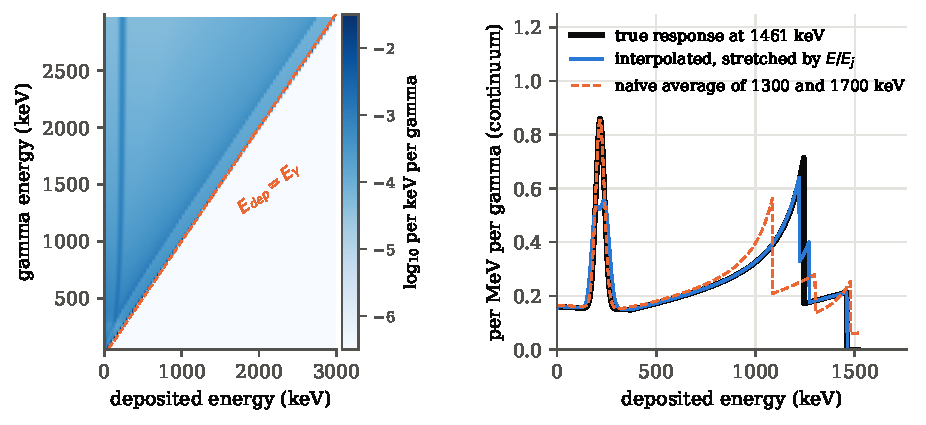
\includegraphics[width=\linewidth]{fig/matrix.pdf}
\caption{Left: a simulated response matrix (here generated from a parameterized model on a \SI{20}{keV} grid of gamma energies). It vanishes above the diagonal $E_\text{dep} = E_\gamma$; the diagonal itself is the photopeak. Right: the continuum response at \SI{1461}{keV} reconstructed from columns simulated at \SIlist{1300;1700}{keV}. Stretching each column by $E/E_j$ (\cref{eq:stretch}) reproduces the true response; averaging the columns produces two false Compton edges.}\label{fig:matrix}
\end{figure}

\paragraph{What the amplitudes mean.} Because a simulated response is per \emph{emitted} photon, the template of \cref{eq:template} is per decay, and the fitted $A_k$ is the number of decays $\mathcal N_k$ during the measurement. Dividing by the live time gives the activity. In the two model-based modes $\varepsilon$ is only relative, so $A_k$ is a decay count times an unknown absolute efficiency, and only the counts $A_k\sum_i T_{ik}$ are meaningful. A small residual efficiency slope $e_1$ (prior $0\pm0.1$) remains free in matrix mode to absorb simulation imperfections.

\begin{exercise}[A]
Prove that the stretched interpolation \cref{eq:stretch} conserves total probability: $\int d(x\mid E)\,\dd x = (1-f)\int d_j + f\int d_{j+1}$.
\end{exercise}

\begin{exercise}[R]
Design the Geant4 simulation that produces a response matrix for a germanium detector in a lead castle, for a source distributed uniformly in the lead. What do you record per event? How many photons per energy do you need so that the matrix's own statistical noise is negligible compared to that of a one-week background spectrum? What changes if you want true-coincidence summing to be included?
\end{exercise}

%=====================================================================
\section{The model of a spectrum and its likelihood}\label{sec:likelihood}
%=====================================================================
\subsection{The model}
The expected counts are
\begin{equation}
\mu_i(\vx,\vth) = \sum_{j} \beta_j B_{ij}(\vth) + \sum_k A_k\,T_{ik}(\vth),\qquad \vx = (\bm\beta,\bm A)\ge 0. \label{eq:model}
\end{equation}
The background is a non-negative combination of cubic B-splines in energy, with $n_\text{knots}$ uniform knots (6--14 by default). This basis is smooth, local, and non-negative. Any non-negative combination is non-negative, so the constraint $\bm\beta\ge0$ yields a physical background. The background stands in for scattered radiation from the surroundings, unmodelled continua (in \code{local} mode, all Compton continua), bremsstrahlung, and anything else without sharp structure.

The model has two kinds of parameters. The vector $\vx$ has dozens of entries: one per candidate source plus the spline weights. $\mu$ is \emph{linear} in them, and they are all non-negative. The vector $\vth$ has 3--15 entries. $\mu$ depends on them \emph{nonlinearly}, through the templates. The algorithm treats the two very differently.

\subsection{The likelihood and the deviance}
From \cref{eq:poisson} the log-likelihood is $\ln L = \sum_i [n_i\ln\mu_i - \mu_i - \ln n_i!]$. It is convenient to compare with the \emph{saturated} model $\mu_i = n_i$, the best any model could do, and define the \emph{deviance}~\cite{BakerCousins}
\begin{equation}
D(\vx,\vth) = -2\ln\frac{L(\vmu)}{L(\vn)} = 2\sum_i\left[\mu_i - n_i + n_i\ln\frac{n_i}{\mu_i}\right]\quad(\text{with } 0\ln 0 = 0). \label{eq:deviance}
\end{equation}
$D\ge0$, each term is non-negative, and for large counts $D \to \sum_i (n_i-\mu_i)^2/\mu_i$, the Pearson $\chi^2$. By Wilks' theorem, at the best fit $D$ is approximately $\chi^2$-distributed with $N - (\text{number of fitted parameters})$ degrees of freedom when the model is correct. So $D/\mathrm{ndf}\approx1$ indicates a good fit, the same intuition as for $\chi^2$. Differences of $D$ between nested models are the likelihood-ratio statistics used for source selection (\cref{sec:selection}).

\begin{pitfall}[Do not fit low-count spectra with least squares]
Minimizing Neyman's $\chi^2_N = \sum(n_i-\mu_i)^2/n_i$ weights downward fluctuations more than upward ones, and biases peak areas low by roughly one count per channel of the peak. Pearson's $\chi^2_P = \sum(n_i-\mu_i)^2/\mu_i$ biases them high. The Poisson likelihood has neither problem, handles empty channels exactly, and costs no more to evaluate. See Baker \& Cousins~\cite{BakerCousins} for the classic analysis.
\end{pitfall}

\paragraph{Deviance residuals.} Define for each channel
\begin{equation}
d_i = \operatorname{sign}(n_i-\mu_i)\sqrt{2\left[\mu_i-n_i+n_i\ln(n_i/\mu_i)\right]},\qquad \textstyle\sum_i d_i^2 = D. \label{eq:devres}
\end{equation}
These behave like Gaussian pulls even at low counts, which is why the fitter plots them under each spectrum. They also turn the Poisson problem into a least-squares problem, which is what Levenberg--Marquardt needs (\cref{sec:theta}).

\subsection{Priors}
Response parameters are rarely unknown. You know the calibration to within a channel or two, and the resolution to tens of percent. The fitter encodes this as independent Gaussian priors and minimizes
\begin{equation}
Q(\vx,\vth) = D(\vx,\vth) + \sum_a \left(\frac{\theta_a-\theta_a^0}{\sigma_a}\right)^2, \label{eq:objective}
\end{equation}
which is $-2\ln$ of the posterior up to a constant, with flat priors on $\vx\ge0$. So the fit result is a \emph{maximum a posteriori} estimate. A parameter with $\sigma_a\to\infty$ is free; one with $\sigma_a = 0$ is fixed. After the fit, the \emph{pull} $(\hat\theta_a-\theta_a^0)/\sigma_a$ is reported. A pull beyond $\pm3$ means the data disagree with what you told the fitter, and usually signals a wrong calibration or detector choice.

\begin{exercise}[A]
Show that minimizing $D$ with respect to an overall scale factor $s$ (all $\mu_i \to s\mu_i$) gives $\sum_i\mu_i = \sum_i n_i$: a Poisson fit always reproduces the total number of counts. Show that the Neyman $\chi^2$ does not, and compute its bias for a flat spectrum with $\mu$ counts per channel.
\end{exercise}

\begin{exercise}[A]
Expand one term of \cref{eq:deviance} to second order in $\delta = n-\mu$ to show $D\to$ Pearson's $\chi^2$. Then compute the third-order term and argue for which counts it can be neglected.
\end{exercise}

%=====================================================================
\section{The linear part: Poisson EM (MLEM)}\label{sec:mlem}
%=====================================================================
For fixed $\vth$, we must solve $\min_{\vx\ge0} D(\vx)$ where $\mu_i = \sum_k T_{ik}x_k$ (folding the splines into $T$). This is a convex problem: $D$ is convex in $\vmu$ and $\vmu$ is linear in $\vx$. But it has dozens of variables, non-negativity constraints, and a non-quadratic objective.

\subsection{Derivation of the EM update}
The expectation-maximization algorithm of Shepp \& Vardi~\cite{SheppVardi} (introduced for emission tomography, which is the same problem) imagines \emph{complete data}: the counts $n_{ik}$ in channel $i$ that came from component $k$, with $n_{ik}\sim\mathrm{Poisson}(T_{ik}x_k)$ and $n_i = \sum_k n_{ik}$. If we knew $n_{ik}$, the maximum-likelihood $x_k$ would be trivial: $\hat x_k = \sum_i n_{ik}/\sum_i T_{ik}$.

\emph{E-step.} Given the current $\vx$, the conditional expectation of $n_{ik}$ given $n_i$ follows from the multinomial split of a Poisson sum:
\begin{equation}
\E[n_{ik}\mid n_i,\vx] = n_i\,\frac{T_{ik}x_k}{\mu_i}.
\end{equation}
\emph{M-step.} Maximize the expected complete-data likelihood, which gives
\begin{equation}
\boxed{\;x_k \leftarrow x_k\;\frac{\sum_i T_{ik}\,n_i/\mu_i}{\sum_i T_{ik}}\;} \label{eq:em}
\end{equation}
This multiplicative update has three remarkable properties.
\begin{enumerate}[nosep]
\item \textbf{Positivity is automatic.} A positive $x_k$ stays positive; no constraint handling is needed.
\item \textbf{Monotonicity.} Every step increases the likelihood (a general EM theorem~\cite{Dempster}), so it cannot diverge.
\item \textbf{The fixed points are the optimality conditions.} At a fixed point either $x_k = 0$ or $\sum_i T_{ik}(1-n_i/\mu_i) = 0$. These are exactly the Karush--Kuhn--Tucker conditions for $\min_{\vx\ge0}D$, because $\partial D/\partial x_k = 2\sum_i T_{ik}(1-n_i/\mu_i)$.
\end{enumerate}
A consequence of property 3 is that the total counts are reproduced exactly at convergence.

\subsection{Acceleration}
Plain EM converges slowly once close to the optimum, because the multiplicative step is small. A common remedy is \emph{over-relaxation}: raise the update factor to a power $\omega>1$,
\begin{equation}
x_k \leftarrow x_k\left(\frac{\sum_i T_{ik}n_i/\mu_i}{\sum_i T_{ik}}\right)^{\omega}.
\end{equation}
The fitter uses $\omega = 1.6$, and then plain EM ($\omega=1$) for the last five iterations to guarantee it ends at a proper EM fixed point. \Cref{fig:mlem} shows the trade-off on a real fit. Over-relaxation speeds up the middle phase. Too large an $\omega$ overshoots, oscillates and diverges. Monotonicity is lost once $\omega>1$, and the guarantee is replaced by testing.

\begin{figure}[tbp]
\centering
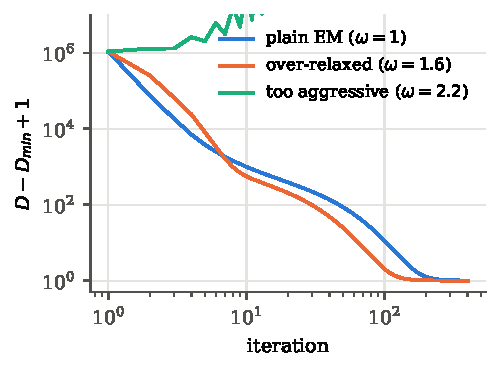
\includegraphics[width=0.48\linewidth]{fig/mlem.pdf}\hfill
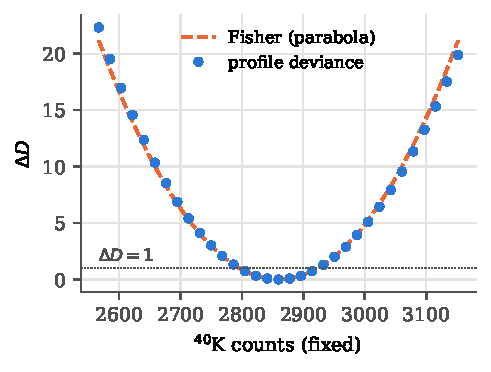
\includegraphics[width=0.48\linewidth]{fig/profile.pdf}
\caption{Left: convergence of the deviance under EM for the HPGe example of \cref{sec:validation} (22 amplitudes, $\vth$ fixed at the truth): plain EM, the over-relaxed version used by the fitter, and an over-aggressive exponent that diverges. Right: profile deviance of the \nuc{40}{K} amplitude (all other amplitudes re-optimized at each point) compared with the parabola implied by the Fisher information (\cref{sec:uncertainty}); for a well-measured peak they agree, and $\Delta D=1$ gives the $1\sigma$ interval.}\label{fig:mlem}
\end{figure}

\subsection{Sparse templates}
A peak template is non-zero over perhaps 20 channels out of 8000. The fitter stores each template as a sparse column \code{\{idx, v, sum\}}: channel indices, values, and the column sum (dropping entries below $10^{-7}$ of the maximum). One EM iteration then costs $\mathcal O(\text{non-zeros})$ instead of $\mathcal O(NK)$.
\begin{lstlisting}[language=JavaScript]
function mlem(cols, data, x, iters) {
  for (var it = 0; it < iters; it++) {
    var mu = model(cols, x, data.length);           // mu = sum_k x_k T_k
    for (var k = 0; k < cols.length; k++) {
      var c = cols[k]; if (!c || !x[k]) continue;
      var num = 0, den = 0;
      for (var i = 0; i < c.v.length; i++) {
        var m = mu[c.idx[i]];
        num += c.v[i] * (m > 0 ? data[c.idx[i]] / m : 0); den += c.v[i];
      }
      x[k] *= Math.pow(num / den, it < iters - 5 ? 1.6 : 1);
    }
  }
  return model(cols, x, data.length);
}
\end{lstlisting}
Note that $\vmu$ is computed once per sweep and all $x_k$ are updated from it (a Jacobi-style sweep). This is the textbook EM. Updating $\vmu$ after each $x_k$ (Gauss--Seidel style) is also valid, often faster, and is what the local refit in \cref{sec:selection} does.

\subsection{Starting values by stripping}\label{sec:start}
EM converges from any positive start, but a good start saves many iterations. The fitter orders sources by the channel where their template peaks, highest energy first. For each source it estimates the amplitude from that template's strongest channels in the current residual, subtracts the source's \emph{whole} template (continuum included), and moves down. Because responses are (nearly) triangular, the highest source's peak region contains nothing from lower sources: this is back substitution. Only 70\% of each estimate is taken, so that the source does not absorb the background under it. Whatever remains is given to the splines.

\begin{exercise}[A]
Starting from the complete-data log-likelihood $\sum_{ik}[n_{ik}\ln(T_{ik}x_k) - T_{ik}x_k]$, carry out the E- and M-steps and derive \cref{eq:em}.
\end{exercise}

\begin{exercise}[A]
Show that if $\vx$ is a fixed point of \cref{eq:em} with all $x_k>0$, then $\sum_i\mu_i = \sum_i n_i$. Then show the KKT statement in property 3.
\end{exercise}

\begin{exercise}[P]
Implement \cref{eq:em} for two overlapping Gaussian peaks on a flat background. Plot the deviance against iteration for $\omega = 1, 1.5, 2$. Then implement the Gauss--Seidel variant and compare. At what peak separation (in units of $\sigma$) does convergence become slow, and why?
\end{exercise}

%=====================================================================
\section{The nonlinear part: response parameters}\label{sec:theta}
%=====================================================================
\subsection{Variable projection}
The full problem is $\min_{\vth}\min_{\vx\ge0}Q(\vx,\vth)$. Rather than fitting $\vx$ and $\vth$ together (dozens of parameters, half of them on constraint boundaries), the fitter \emph{eliminates} $\vx$:
\begin{equation}
\tilde Q(\vth) = \min_{\vx\ge0} Q(\vx,\vth), \label{eq:varpro}
\end{equation}
evaluating $\tilde Q$ by running EM, and minimizes $\tilde Q$ over the few $\vth$. This is the \emph{variable projection} idea of Golub \& Pereyra~\cite{GolubPereyra}. The outer problem is small and smooth. The inner problem is convex and solved by a robust special-purpose method. Warm-starting each EM from the previous $\vx$ makes inner solves cheap.

\subsection{Levenberg--Marquardt on deviance residuals}
Write the objective as a sum of squares, $\tilde Q(\vth) = \|\bm r(\vth)\|^2$, with residual vector
\begin{equation}
\bm r = \big(d_1,\dots,d_N,\; (\theta_1-\theta_1^0)/\sigma_1,\dots\big),
\end{equation}
the deviance residuals of \cref{eq:devres} followed by the prior pulls. With Jacobian $J_{ia} = \partial r_i/\partial\theta_a$, Gauss--Newton linearizes $\bm r(\vth+\bm\delta)\approx\bm r+J\bm\delta$ and solves $J\T J\,\bm\delta = -J\T\bm r$. Levenberg~\cite{Levenberg} and Marquardt~\cite{Marquardt} added damping:
\begin{equation}
\left(J\T J + \lambda\,\mathrm{diag}(J\T J)\right)\bm\delta = -J\T\bm r. \label{eq:lm}
\end{equation}
Small $\lambda$ gives Gauss--Newton (fast near the minimum). Large $\lambda$ gives a short, scaled gradient step (safe far away). After each trial step the fitter re-solves the amplitudes and recomputes $\tilde Q$. It accepts the step only if $\tilde Q$ decreased, and then divides $\lambda$ by 5. Otherwise it multiplies $\lambda$ by 8 and tries again (up to six times). It stops when $\tilde Q$ improves by less than 0.05 or after 25 iterations.

\subsection{The Jacobian with fixed amplitudes}
The exact Jacobian of the projected residuals includes $\partial\hat{\vx}/\partial\vth$, the change of the optimal amplitudes. Kaufman~\cite{Kaufman} showed that dropping that term (holding $\vx$ fixed while differentiating) costs little: the gradient is still exact at the optimum, by the envelope theorem $\nabla\tilde Q = \partial Q/\partial\vth|_{\hat{\vx}}$, and only the curvature estimate is approximate. The fitter takes forward differences with step $0.05\,\sigma_a$:
\begin{lstlisting}[language=JavaScript]
for (var j = 0; j < P; j++) {
  var k = this.free[j], h = 0.05 * o.params[k].sigma, q = Object.assign({}, p); q[k] += h;
  var bq = this.build(q, srcs);                        // templates at theta + h e_j
  var rr = { mu: model(bq.cols, cur.x, this.data.length) };   // amplitudes held fixed
  var rv = resid(rr, q);
  for (var i = 0; i < nres; i++) col[i] = (rv[i] - r0[i]) / h;
}
\end{lstlisting}
Holding $\vx$ fixed also makes the derivatives \emph{noise-free}. An earlier version re-solved EM inside each finite difference, and the slight non-convergence of EM made the Jacobian noisy enough to stall the iteration.

\begin{keyidea}[Why priors make the problem well posed]
Without priors, parameters can be degenerate. With only one peak in the range, the calibration offset and gain cannot both be determined, and $J\T J$ is singular. The prior rows of $\bm r$ add $1/\sigma_a^2$ to the diagonal of $J\T J$, so it is always invertible. Each parameter is then determined by the data where the data have something to say and by the prior otherwise. This also explains a result in \cref{sec:validation}: when the truth has a resolution term ($cE^2$) that the fit holds fixed at zero, the correlated $b$ term absorbs it, and $b$ is pulled several standard errors from its true value while the fit stays good.
\end{keyidea}

\begin{exercise}[A]
Show that for $\lambda\to0$ \cref{eq:lm} is the Gauss--Newton step and for $\lambda\to\infty$ it is a gradient-descent step of length $\propto1/\lambda$. Why is the scaling by $\mathrm{diag}(J\T J)$ (Marquardt) better than adding $\lambda\mathbb 1$ (Levenberg) when parameters have very different units, such as $c_0$ in keV and the dimensionless $c$?
\end{exercise}

\begin{exercise}[A]
Prove the envelope-theorem statement: if $\hat{\vx}(\vth)$ minimizes $Q(\cdot,\vth)$ and is differentiable (interior solution), then $\dd\tilde Q/\dd\vth = \partial Q/\partial\vth$ at $\hat{\vx}$. What changes for an amplitude stuck at the boundary $x_k=0$?
\end{exercise}

\begin{exercise}[P]
Extend your two-peak code from \cref{sec:mlem} to fit the calibration $(c_0,c_1)$ and resolution $(a,b)$ by Levenberg--Marquardt with priors, re-solving amplitudes by EM at each trial step. Compare with \code{minifit.py} (\cref{app:minifit}).
\end{exercise}

%=====================================================================
\section{Choosing the sources}\label{sec:selection}
%=====================================================================
\subsection{The candidate list and its prior}
The Gamma Line Explorer ranks every source in its database (decays, neutron capture and inelastic lines, ($\alpha$,x) reactions, cosmogenic activation) by an expected rate for the user's setup. It then hands the top $N$ (60 by default) that have lines in the fit range to the fitter. Each gets a prior probability from its rank,
\begin{equation}
\pi_k = \max\!\left(10^{-4},\;\sqrt{\text{rate}_k/\text{rate}_\text{top}}\right),
\end{equation}
so the most expected source has $\pi=1$ and one eight decades down has $\pi = 10^{-4}$.

\subsection{Likelihood-ratio test for one source}
Should source $k$ be in the model? Compare the best fit with and without it:
\begin{equation}
\Delta D_k = D_{\text{without }k} - D_{\text{with }k} \ge 0.
\end{equation}
If the source is absent, $\Delta D_k$ is distributed as $\tfrac12\chi^2_0 + \tfrac12\chi^2_1$ (Chernoff~\cite{Chernoff}). This is a half-and-half mixture rather than $\chi^2_1$, because the amplitude is bounded at zero and half of the time the best fit puts it there. So $\sqrt{\Delta D_k}$ is approximately the significance in Gaussian standard deviations. This is the ``Significance'' column the page reports.

\subsection{A prior-dependent threshold}
Source $k$ is kept only if
\begin{equation}
\Delta D_k > \tau + 2\ln(1/\pi_k),\qquad \tau = 9 \text{ by default}. \label{eq:threshold}
\end{equation}
The term $2\ln(1/\pi_k)$ has a Bayesian reading. The posterior odds for including the source are the likelihood ratio $e^{\Delta D/2}$ times the prior odds $\approx\pi_k$. Requiring the posterior odds to exceed $e^{\tau/2}$ gives exactly \cref{eq:threshold}. An unlikely isotope ($\pi=10^{-4}$) therefore needs $\Delta D > 27.4$, about $5.2\sigma$, while \nuc{40}{K} needs only $3\sigma$. This is the explorer's encoding of ``extraordinary claims require extraordinary evidence''. It also tames the look-elsewhere effect: with 60 candidates, a flat $3\sigma$ cut would let through a false source every few fits.

\subsection{Backward elimination}
The fitter starts with all candidates and removes them, as in \cref{alg:elim}. Forward selection (adding sources one at a time) would be cheaper per step. But it fails when two sources share lines (for example \nuc{214}{Pb} and \nuc{214}{Bi}, or members of a chain): neither looks significant alone until the other is present.

\begin{algorithm}[t]
\caption{Source selection by backward elimination}\label{alg:elim}
\KwIn{candidates $\mathcal K$ with priors $\pi_k$; current solution $(\vx,\vth)$}
\Repeat{nothing is dropped}{
  \lForEach{$k\in\mathcal K$}{compute the removal cost $\Delta D_k$ (local refit, see text)}
  $\mathcal E \leftarrow \{k : \Delta D_k < 1\}$ \tcp*{sources the fit gives (almost) nothing to}
  \eIf{$\mathcal E \neq \emptyset$}{remove all of $\mathcal E$}{
    $k^\star \leftarrow \arg\min_k\,[\Delta D_k - \tau - 2\ln(1/\pi_k)]$\;
    \lIf{that minimum is $<0$}{remove $k^\star$ \textbf{else} stop}
  }
  re-solve the amplitudes by EM (warm start)\;
}
\end{algorithm}

The whole fit (\code{run}) is: eliminate with the starting $\vth$; fit $\vth$ by Levenberg--Marquardt with the surviving sources; eliminate again with the fitted response; final EM and uncertainties (\cref{fig:flow}).

\paragraph{Local removal cost.} Computing $\Delta D_k$ exactly needs a full refit without source $k$, once per source per round, which is too slow in a browser. The fitter instead refits only the channels where source $k$'s template is non-zero, and only the columns that overlap them, with 30 Gauss--Seidel EM sweeps. The other channels keep their full-fit values. This is accurate whenever sources' influences are local, which is the case for peaks. An earlier version refitted the entire spectrum. That was not only slower but worse: the background splines could reshape themselves far from the peak and absorb part of the cost.

\begin{figure}[tbp]
\centering
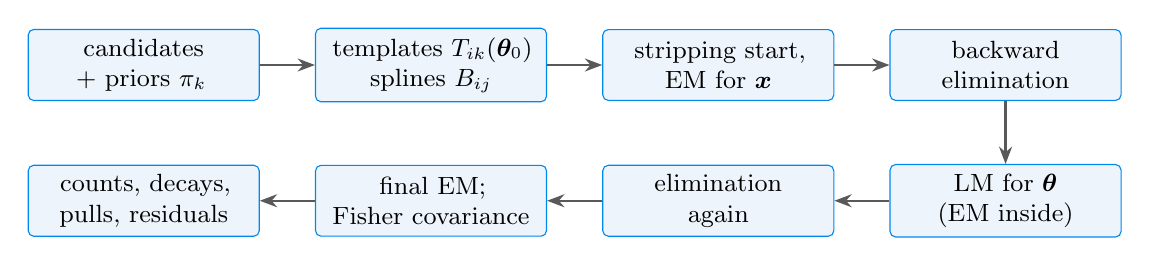
\begin{tikzpicture}[node distance=5mm and 7mm, every node/.style={font=\small},
  box/.style={draw=labblue,fill=boxbg,rounded corners=2pt,align=center,minimum height=9mm,text width=27mm},
  arr/.style={-{Stealth[length=2.2mm]},thick,draw=black!65}]
\node[box] (c) {candidates\\+ priors $\pi_k$};
\node[box,right=of c] (t) {templates $T_{ik}(\vth_0)$\\splines $B_{ij}$};
\node[box,right=of t] (s) {stripping start,\\EM for $\vx$};
\node[box,right=of s] (e1) {backward\\elimination};
\node[box,below=8mm of e1] (lm) {LM for $\vth$\\(EM inside)};
\node[box,left=of lm] (e2) {elimination\\again};
\node[box,left=of e2] (f) {final EM;\\Fisher covariance};
\node[box,left=of f] (o) {counts, decays,\\pulls, residuals};
\draw[arr] (c)--(t); \draw[arr] (t)--(s); \draw[arr] (s)--(e1); \draw[arr] (e1)--(lm); \draw[arr] (lm)--(e2); \draw[arr] (e2)--(f); \draw[arr] (f)--(o);
\end{tikzpicture}
\caption{The sequence of steps in one fit (\code{run} in \code{gammafit-core.js}).}\label{fig:flow}
\end{figure}

\begin{exercise}[P]
Verify Chernoff's result by toy Monte Carlo. Simulate 2000 spectra of a flat background only, fit each with and without a Gaussian peak of fixed position and width (amplitude $\ge0$), and histogram $\Delta D$. What fraction is exactly zero? Compare the tail with $\tfrac12\chi^2_1$.
\end{exercise}

\begin{exercise}[R]
Now let the peak position float over the whole range. How does the distribution of $\Delta D$ change? Estimate the trials factor and relate it to the prior penalty $2\ln(1/\pi)$. (This is the look-elsewhere effect.)
\end{exercise}

\begin{exercise}[A]
Show that \cref{eq:threshold} with $\tau = 2\ln 10 \approx 4.6$ and $\pi = 1$ is equivalent to requiring the Bayes factor to exceed 10, and relate $\tau$ to the AIC ($\tau=2$) and BIC ($\tau=\ln N$) penalties for one extra parameter.
\end{exercise}

%=====================================================================
\section{Uncertainties}\label{sec:uncertainty}
%=====================================================================
\subsection{Fisher information}
Near the optimum, $\tfrac12 Q$ is approximately quadratic in all parameters $\bm q = (\vx_\text{active},\vth)$. Its expected Hessian is the Fisher information
\begin{equation}
F_{ab} = \sum_i \frac{1}{\mu_i}\frac{\partial\mu_i}{\partial q_a}\frac{\partial\mu_i}{\partial q_b} + \delta_{ab}\,\frac{[a\in\vth]}{\sigma_a^2},\qquad \mathrm{Cov}(\hat{\bm q}) \approx F^{-1}. \label{eq:fisher}
\end{equation}
For an amplitude, $\partial\mu_i/\partial A_k = T_{ik}$, available directly. For a response parameter, the derivative is a finite difference of the model. The fitter builds the joint matrix over all active amplitudes \emph{and} free $\vth$ and inverts it (\code{covariance}). A source's uncertainty therefore includes its correlation with the resolution, calibration or peak-to-total ratio. This matters most in Compton mode, where the continuum shape trades off against the background.

The reported counts are $A_k\sum_iT_{ik}$, with uncertainty $\sigma_{A_k}\sum_iT_{ik}$. The reported decays (matrix mode) are $A_k\pm\sigma_{A_k}$.

\subsection{When the parabola fails}
\Cref{fig:mlem} (right) checks \cref{eq:fisher} against a profile scan for a well-measured peak; they agree. The approximation fails for weak sources near the boundary, where the profile is one-sided, and for strongly nonlinear parameters. The honest alternatives are a profile-likelihood interval, where $\Delta D = 1$ gives $1\sigma$, or for upper limits a Feldman--Cousins construction. A further option is to sample the posterior $\propto e^{-Q/2}$ by Markov-chain Monte Carlo. All are natural extensions (\cref{sec:limits}).

\subsection{What the uncertainties do not include}
The quoted uncertainties are statistical, plus whatever the priors and response parameters propagate. They do \emph{not} include several things: errors in the shape of the response model, the systematic difference between Compton mode and a true response (\cref{sec:validation}), nuclear-data uncertainties on line intensities, true-coincidence summing, and in matrix mode the simulation's geometry and materials.

\begin{exercise}[A]
For a single Gaussian peak of area $A$ on a flat background $b$ per channel, derive $\sigma_A^2$ from \cref{eq:fisher} in the limits $A\gg b\cdot\mathrm{FWHM}$ and $A\ll b\cdot\mathrm{FWHM}$. Recover the familiar rule that a peak's significance grows as $A/\sqrt{b\,\mathrm{FWHM}}$, and estimate the optimal window width for a simple counting analysis.
\end{exercise}

\begin{exercise}[P]
Use \code{minifit.py}'s toy Monte Carlo to check the coverage of the quoted uncertainties: the pulls $(\hat A-A_\text{true})/\sigma_A$ should have mean 0 and width 1. Reduce the \nuc{137}{Cs} amplitude until the pull distribution visibly deviates. Explain what you see.
\end{exercise}

%=====================================================================
\section{Implementation notes}\label{sec:implementation}
%=====================================================================
\paragraph{Structure.} \code{gammafit-core.js} is organized as follows.
\begin{itemize}[nosep]
\item Physics helpers: \code{energyOf}, \code{fwhm}, \code{eff}, \code{peakToTotal}, \code{kn}, \code{knNorm}, \code{erfc}.
\item The channel geometry: \code{Grid}, with a binary search from energy to fractional channel.
\item Template builders: \code{addGauss}, \code{addStepTail}, \code{smear}, \code{template}, \code{matSource} and \code{matTemplate}.
\item Linear algebra for small systems: \code{solve}, \code{invert}.
\item The \code{Fit} object, with methods \code{build}, \code{linear}, \code{strip}, \code{prior}, \code{objective}, \code{fitTheta}, \code{removalCost} and \code{covariance}.
\item The driver \code{run}.
\end{itemize}
The same file runs as a Web Worker in the page (so the interface stays responsive) and as a Node module in tests.

\paragraph{Numerical care.}
\begin{itemize}[nosep]
\item $\mu_i$ is clamped at $10^{-12}$ inside logarithms, and $0\ln0 = 0$ is handled explicitly.
\item The Fisher matrix uses $\max(\mu_i,1)$ in the denominator, to avoid huge weights from channels with tiny expectation.
\item \code{erfc} uses a Chebyshev-fitted rational approximation with relative error $<1.2\times10^{-7}$.
\item Resolution smearing normalizes each Gaussian kernel over the grid, so that smearing conserves counts.
\item Since only $a^2$ enters \cref{eq:fwhm}, a negative fitted $a$ is folded to $|a|$.
\item A step that makes $c_1\le0$ is rejected.
\end{itemize}

\paragraph{Cost.} Building templates dominates: each LM iteration builds $P$ perturbed template sets, each with $K$ templates. With sparse columns and the local removal cost, a fit of an 8192-channel HPGe spectrum with 60 candidates takes 1--3\,s in a browser. Matrix mode caches the unsmeared responses, so it costs about the same as Compton mode.

\paragraph{Testing.} The fitter was developed against \emph{closure tests}: synthesize a spectrum from known sources with the same template code plus Poisson noise, fit it, and compare with the truth. Closure tests check the algorithm, not the physics. They are necessary but not sufficient, and \cref{sec:validation} shows both what they establish and what they cannot.

\begin{exercise}[P]
Profile the fitter in Node (\code{node --prof}) on the HPGe example. Which functions dominate? Propose and implement one optimization (for example, analytic derivatives of the Gaussian templates with respect to $c_0$, $c_1$, $a$, $b$) and measure the gain.
\end{exercise}

%=====================================================================
\section{Validation on simulated spectra}\label{sec:validation}
%=====================================================================
\subsection{HPGe, \code{local} mode}
An 8192-channel HPGe spectrum was simulated with \nuc{226}{Ra}, \nuc{228}{Th} and \nuc{228}{Ac} chain segments and \nuc{40}{K}, on an exponential background. It was fitted from \SI{150}{keV} with eight candidates (adding \nuc{60}{Co}, \nuc{137}{Cs}, \nuc{235}{U} and \nuc{54}{Mn} as decoys) and nine free response parameters. \Cref{tab:hpge} and \cref{fig:fith} show the result. All four true sources are found, all four decoys are rejected, and the counts agree with the truth within about $1\sigma$. The fit took \SI{1.3}{s} in Node. The resolution term $b$ comes out at $0.00223\pm0.00004$ against a true 0.0019. The simulation included a small $cE^2$ term that the fit held fixed at zero, and $b$ absorbed it ($cE\approx3\times10^{-4}$ at \SI{1.5}{MeV}). The fit quality is unaffected ($D/\mathrm{ndf} = 8108/7763 = 1.04$).

\begin{table}[h]
\centering\small
\caption{HPGe closure test (counts in the fit range).}\label{tab:hpge}
\begin{tabular}{@{}lrrrr@{}}
\toprule
Source & True counts & Fitted counts & $\sigma$ & $\sqrt{\Delta D}$\\
\midrule
\nuc{226}{Ra} segment & \num{53584} & \num{53173} & 408 & 317\\
\nuc{228}{Th} segment & \num{24039} & \num{24069} & 320 & 189\\
\nuc{228}{Ac} & \num{8852} & \num{8764} & 134 & 90\\
\nuc{40}{K} & \num{2793} & \num{2841} & 66 & 69\\
\nuc{60}{Co}, \nuc{137}{Cs}, \nuc{235}{U}, \nuc{54}{Mn} & 0 & removed & & \\
\bottomrule
\end{tabular}
\end{table}

\begin{figure}[tbp]
\centering
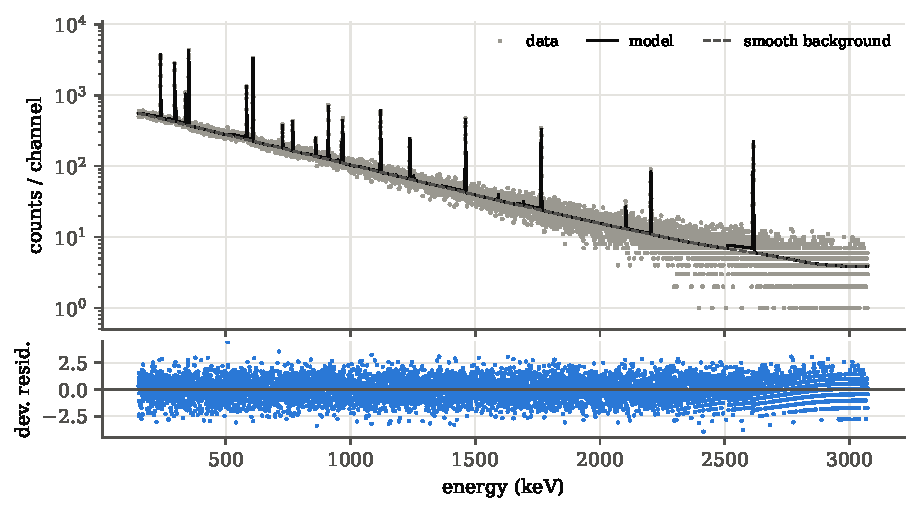
\includegraphics[width=\linewidth]{fig/fit_hpge_full.pdf}\\[2pt]
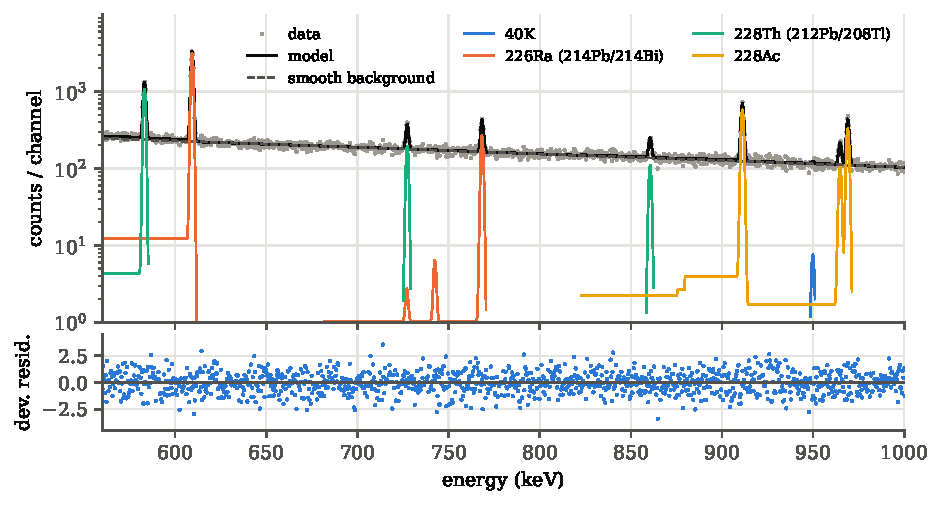
\includegraphics[width=\linewidth]{fig/fit_hpge.pdf}
\caption{HPGe closure test. Top: whole fit range with data, model and smooth background. Bottom: zoom on \SIrange{560}{1000}{keV} with the individual source components; the step under each peak is visible. Deviance residuals are below each panel.}\label{fig:fith}
\end{figure}

\subsection{A scintillator: simulated response versus Compton model}
A 1024-channel spectrum with scintillator-like resolution (FWHM$\,\approx\,$\SI{70}{keV} at \SI{1.5}{MeV}) was simulated from the response matrix of \cref{fig:matrix} with $1.2\times10^6$ \nuc{226}{Ra}, $8\times10^5$ \nuc{228}{Th} and $2\times10^6$ \nuc{40}{K} decays. It was then fitted twice: with the same matrix (matrix mode), and with the parameterized Compton model, which does \emph{not} match how the data were made (\cref{tab:nai,fig:fitn}).

\begin{table}[h]
\centering\small
\caption{Scintillator test: the same spectrum fitted with the simulated response and with the Compton model.}\label{tab:nai}
\begin{tabular}{@{}lrrrrr@{}}
\toprule
& \multicolumn{2}{c}{Matrix mode} & & \multicolumn{2}{c}{Compton mode}\\
\cmidrule{2-3}\cmidrule{5-6}
Source & Decays (true) & Decays (fit) & True counts & Counts (fit) & Bias\\
\midrule
\nuc{226}{Ra} & \num{1200000} & $\num{1201600}\pm\num{2900}$ & \num{1170405} & $\num{1096000}\pm\num{6300}$ & $-6.4\%$\\
\nuc{228}{Th} & \num{800000} & $\num{801500}\pm\num{2600}$ & \num{649761} & $\num{593800}\pm\num{3900}$ & $-8.6\%$\\
\nuc{40}{K} & \num{2000000} & $\num{1993000}\pm\num{15600}$ & \num{106940} & $\num{100400}\pm\num{900}$ & $-6.1\%$\\
\midrule
$D/\mathrm{ndf}$ & & $1310/967$ & & $3235/962$ & \\
\bottomrule
\end{tabular}
\end{table}

\begin{figure}[tbp]
\centering
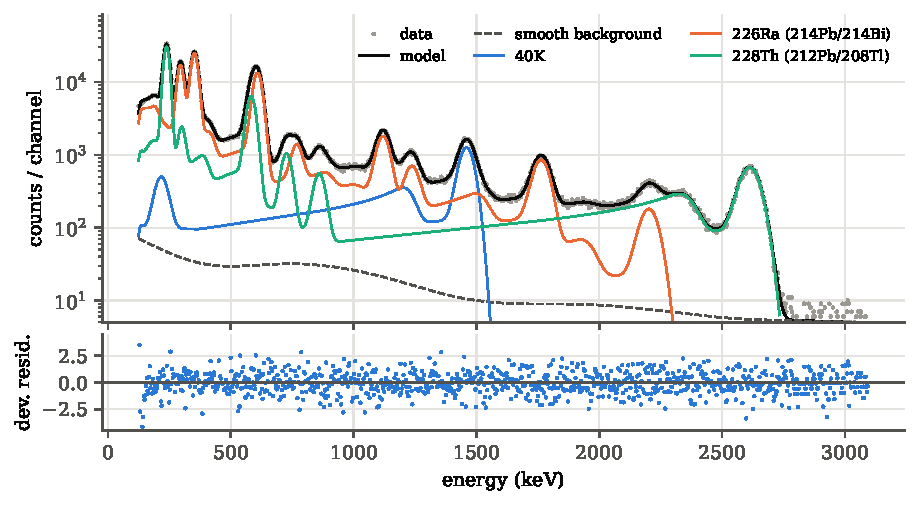
\includegraphics[width=\linewidth]{fig/fit_matrix.pdf}\\[2pt]
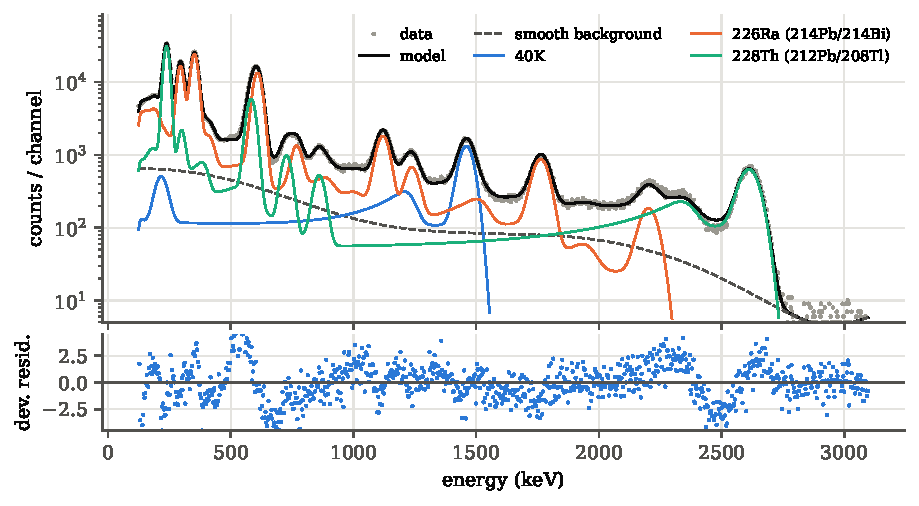
\includegraphics[width=\linewidth]{fig/fit_compton.pdf}
\caption{Scintillator test. Top: matrix mode, residuals flat. Bottom: Compton mode on the same data; the structured residuals around the Compton edges and the poorer deviance show the model mismatch.}\label{fig:fitn}
\end{figure}

The matrix fit recovers the number of decays to within $0.4\%$ ($\le0.6\sigma$) and needs no efficiency calibration. The Compton-model fit is visibly worse in its residuals, and its counts are biased by 6--9\%, several times the quoted statistical uncertainty. This is the systematic error of a semi-empirical response, and it is why the matrix option exists. The matrix fit's own $D/\mathrm{ndf} = 1.35$ is also above 1. The cause is interpolation between \SI{20}{keV} columns and resampling the \SI{2}{keV} deposit grid onto \SI{3}{keV} channels. It is a reminder that every response is an approximation.

\begin{exercise}[R]
Take a real spectrum from the lab (a \nuc{228}{Th} or \nuc{137}{Cs} calibration in one of our scintillators). Fit it in Compton mode, calibrating the peak-to-total ratio and shelf. Then build a Geant4 response for the same geometry and fit it in matrix mode. Quantify the difference in fitted counts, and decide which you would trust for an activity measurement and why.
\end{exercise}

%=====================================================================
\section{Limits and extensions}\label{sec:limits}
%=====================================================================
\begin{itemize}
\item \textbf{True-coincidence summing.} Cascades (\nuc{60}{Co}, \nuc{214}{Bi}, \nuc{208}{Tl}) in close geometry lose counts from photopeaks and create sum peaks. A simulation that emits whole decays (not single photons) includes this automatically. The decay-chain tab already lists which gammas are emitted together.
\item \textbf{Nonlinearity.} Scintillators are not perfectly proportional (Birks quenching, the NaI(Tl) non-proportionality). The quadratic calibration term is only a crude stand-in.
\item \textbf{Light-yield parameterization.} Tying the statistical resolution term to the gain, $b = 5.55f\,c_1$ for an axis in photoelectrons, would make each peak's width constrain the energy scale too.
\item \textbf{Pile-up and dead time} at high rates. \textbf{X-ray escape peaks} in NaI and Ge. A full \textbf{efficiency curve below \SI{100}{keV}}.
\item \textbf{Full posterior sampling} (MCMC over $\vth$ with EM for $\vx$, or Hamiltonian Monte Carlo over all) for honest intervals on weak sources.
\item \textbf{Background modelling.} Splines are agnostic. A physics-based background, such as a simulated cosmic or radon contribution, could replace part of them.
\end{itemize}

%=====================================================================
\section{Capstone project}\label{sec:capstone}
%=====================================================================
\begin{exercise}[R, several weeks]
Build, validate and apply your own forward-folding fitter.
\begin{enumerate}[nosep,label=(\alph*)]
\item Implement templates for one detector type you work with, from \cref{eq:local} or \cref{eq:compton-model}, with bin-integrated peaks.
\item Implement EM for the amplitudes and Levenberg--Marquardt with priors for the response, as in \code{minifit.py}, but with a candidate list from the Gamma Line Explorer (export its CSV).
\item Validate by closure tests: bias and pull distributions for every amplitude over 500 toys, at high and at low statistics.
\item Implement backward elimination with the threshold of \cref{eq:threshold}. Measure the false-source rate on background-only toys, and the efficiency for a weak injected source, as functions of $\tau$.
\item Apply it to a real assay spectrum from the lab's HPGe detector, compare with the web fitter, and write a two-page note on the activities and their uncertainties, including systematics.
\end{enumerate}
\end{exercise}

%=====================================================================
\appendix
\section{Parameters and default priors}\label{app:params}
%=====================================================================
\begin{table}[h]
\centering\small
\caption{Response parameters (\code{PNAMES}) and the defaults set by the page. $f_1$ is the detector's FWHM at \SI{1}{MeV} chosen in the setup; ``fixed'' means not fitted unless the user frees it.}
\begin{tabularx}{\linewidth}{@{}llX@{}}
\toprule
Name & Meaning & Default prior\\
\midrule
\code{c0}, \code{c1}, \code{c2} & calibration \cref{eq:calib} & from the file's axis or the user's calibration; $\sigma_{c_0}=\max(0.5,f_1)$\,keV, $\sigma_{c_1}=0.3\%$; $c_2$ fixed\\
\code{a}, \code{b}, \code{c} & resolution \cref{eq:fwhm} & HPGe: $a=0.55f_1\pm0.3f_1$, $b=0.7f_1^2/1000\pm50\%$, $c$ fixed; others: $a=0.05f_1\pm0.1f_1$, $b=f_1^2/1000\pm40\%$, $c=0\pm0.2f_1^2/10^6$\\
\code{e1}, \code{e2} & efficiency \cref{eq:eff} & $e_1=-0.8$ (HPGe) or $-0.6\pm0.4$; $e_2=-0.1\pm0.2$; matrix mode $e_1=0\pm0.1$, $e_2$ fixed\\
\code{step} & HPGe step height (fraction of peak height) & $0.003\pm0.003$ (local and HPGe matrix mode)\\
\code{tail}, \code{tailw} & exponential tail fraction and slope ($\sigma$ units) & fixed at 0 and 1\\
\code{se}, \code{de} & escape fractions at \SI{2614}{keV} & $0.05\pm0.05$, $0.02\pm0.02$ (local mode)\\
\code{pt}, \code{ptk} & $P/T$ at \SI{662}{keV} and its power-law index & $0.5\pm0.25$ ($0.7$ for liquid nobles), $0.6\pm0.3$ (Compton mode)\\
\code{shelf}, \code{bs} & shelf and backscatter shares of the non-peak part & $0.15\pm0.1$, $0.05\pm0.05$ (Compton mode)\\
\bottomrule
\end{tabularx}
\end{table}

\section{A minimal fitter in Python}\label{app:minifit}
\code{minifit.py} (in \code{docs/gammafit/}) implements bin-integrated Gaussian templates, a two-function non-negative background, EM, Levenberg--Marquardt with priors and variable projection, Fisher uncertainties, and a toy-MC coverage check, for \nuc{137}{Cs} and \nuc{60}{Co} lines. Its output:
\lstinputlisting[basicstyle=\ttfamily\scriptsize]{minifit_output.txt}
The full listing follows. Read it alongside \cref{sec:mlem,sec:theta,sec:uncertainty}.
\lstinputlisting[language=Python,basicstyle=\ttfamily\scriptsize]{minifit.py}

%=====================================================================
\begin{thebibliography}{99}
\bibitem{KleinNishina} O.~Klein and Y.~Nishina, ``\"Uber die Streuung von Strahlung durch freie Elektronen nach der neuen relativistischen Quantendynamik von Dirac,'' Z.~Phys.\ \textbf{52}, 853 (1929).
\bibitem{Knoll} G.~F.~Knoll, \emph{Radiation Detection and Measurement}, 4th ed.\ (Wiley, 2010), chapters 10 and 12.
\bibitem{PhillipsMarlow} G.~W.~Phillips and K.~W.~Marlow, ``Automatic analysis of gamma-ray spectra from germanium detectors,'' Nucl.\ Instrum.\ Meth.\ \textbf{137}, 525 (1976).
\bibitem{BakerCousins} S.~Baker and R.~D.~Cousins, ``Clarification of the use of chi-square and likelihood functions in fits to histograms,'' Nucl.\ Instrum.\ Meth.\ \textbf{221}, 437 (1984).
\bibitem{SheppVardi} L.~A.~Shepp and Y.~Vardi, ``Maximum likelihood reconstruction for emission tomography,'' IEEE Trans.\ Med.\ Imaging \textbf{1}, 113 (1982).
\bibitem{Dempster} A.~P.~Dempster, N.~M.~Laird and D.~B.~Rubin, ``Maximum likelihood from incomplete data via the EM algorithm,'' J.~R.\ Stat.\ Soc.\ B \textbf{39}, 1 (1977).
\bibitem{Levenberg} K.~Levenberg, ``A method for the solution of certain non-linear problems in least squares,'' Q.~Appl.\ Math.\ \textbf{2}, 164 (1944).
\bibitem{Marquardt} D.~W.~Marquardt, ``An algorithm for least-squares estimation of nonlinear parameters,'' J.~SIAM \textbf{11}, 431 (1963).
\bibitem{GolubPereyra} G.~H.~Golub and V.~Pereyra, ``The differentiation of pseudo-inverses and nonlinear least squares problems whose variables separate,'' SIAM J.\ Numer.\ Anal.\ \textbf{10}, 413 (1973).
\bibitem{Kaufman} L.~Kaufman, ``A variable projection method for solving separable nonlinear least squares problems,'' BIT \textbf{15}, 49 (1975).
\bibitem{Chernoff} H.~Chernoff, ``On the distribution of the likelihood ratio,'' Ann.\ Math.\ Stat.\ \textbf{25}, 573 (1954).
\bibitem{FeldmanCousins} G.~J.~Feldman and R.~D.~Cousins, ``Unified approach to the classical statistical analysis of small signals,'' Phys.\ Rev.\ D \textbf{57}, 3873 (1998).
\bibitem{Geant4} S.~Agostinelli \emph{et al.}\ (Geant4), ``Geant4---a simulation toolkit,'' Nucl.\ Instrum.\ Meth.\ A \textbf{506}, 250 (2003).
\end{thebibliography}
\end{document}
